\section{Servers}

Servers housed within individual shelves form the foundational components of warehouse-scale computers. 
These servers are interconnected through hierarchical networks and are sustained by a shared power and cooling infrastructure.

They resemble standard PCs but are designed with form factors that enable them to fit into shelves, such as rack (one or more), blade enclosure format, or tower configurations. 
Servers are typically constructed in a tray or blade enclosure format, housing the motherboard, chipset, and additional plug-in components.

\paragraph*{Motherboard}
The motherboard offers sockets and plug-in slots for installing CPUs, memory modules (DIMMs), local storage (such as Flash SSDs or HDDs), and network interface cards (NICs) to meet various resource requirements.

The chipset and additional components of these systems include:
\begin{itemize}
    \item \textit{Number and type of CPUs}: these systems support a varying number of CPU sockets, typically ranging from 1 to 8, and can accommodate processors such as Intel Xeon Family, AMD EPYC, etc.
    \item \textit{Available RAM}: they offer a range of DIMM slots, typically from 2 to 192, for memory modules.
    \item \textit{Locally attached disks}: these systems come with between 1 and 24 drive bays for local storage. 
        They support both HDD and SSD options, with specific configurations detailed in lectures. 
        Users can choose between SAS for higher performance (albeit at a higher cost) or SATA for entry-level servers.
    \item \textit{Other special purpose devices}: these systems can integrate specialized components like GPUs or TPUs, with support for various models including NVIDIA Pascal, Volta, A100, etc.
    \item \textit{Form factor}: they come in different sizes, ranging from 1U to 10U, and can also be configured as tower systems.
\end{itemize}

\subsection{Racks}
Racks serve as specialized shelves designed to house and interconnect all IT equipment. 
They are utilized for storing rack servers and are measured in rack units, denoted as U, with one rack unit (1U) equivalent to 44.45 mm (1.75 inches). 
One of the advantages of using racks is that they allow designers to stack additional electronic devices alongside the servers.
IT equipment must adhere to specific sizes to fit into the rack shelves.
\begin{figure}[H]
    \centering
    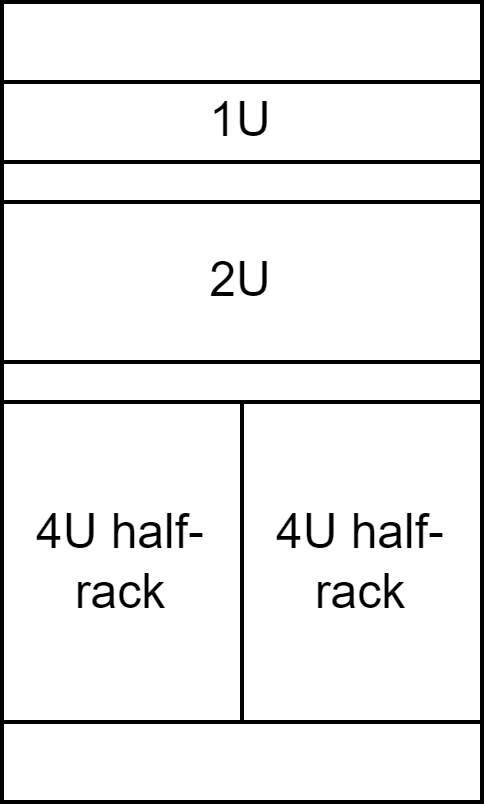
\includegraphics[width=0.2\linewidth]{images/rack.png}
    \caption{Rack elements dimensions}
\end{figure}
The rack serves as the shelf that securely holds together tens of servers.
It manages the shared power infrastructure, including power delivery, battery backup, and power conversion. 
The width and depth of racks vary across WSCs, with some adhering to classic 19-inch width and 48-inch depth, while others may be wider or shallower. 
It is often convenient to connect network cables at the top of the rack, leading to the adoption of rack-level switches appropriately called Top of Rack (TOR) switches.
\begin{figure}[H]
    \centering
    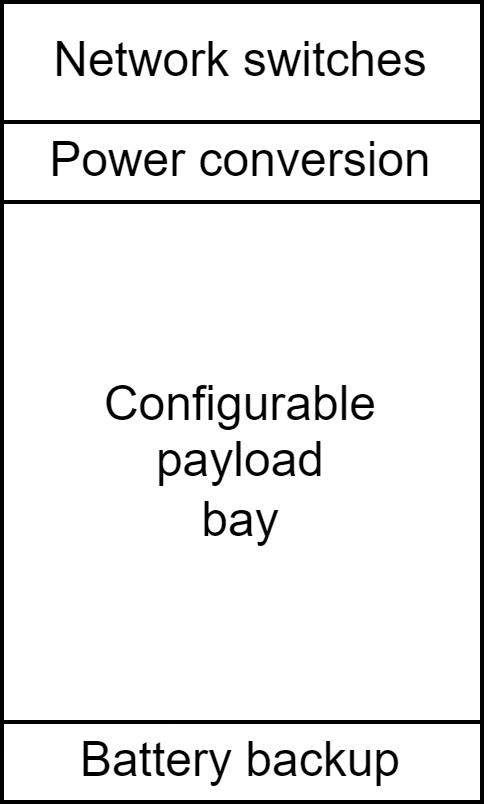
\includegraphics[width=0.2\linewidth]{images/rack1.png}
    \caption{Rack structure}
\end{figure}
Advantages of using racks include the ease of failure containment, as identifying and replacing malfunctioning servers is a straightforward process. 
Additionally, racks offer simplified cable management, making it efficient to organize cables. 
Moreover, they provide cost-effectiveness by offering computing power and efficiency at relatively lower costs.

However, there are also drawbacks to consider. The high overall component density within racks leads to increased power usage, requiring additional cooling systems. 
Consequently, this results in higher power consumption. 
Furthermore, maintaining multiple devices within racks becomes considerably challenging as the number of racks increases, making maintenance a complex task.

\subsection{Towers}
A tower server closely resembles a traditional tower PC in appearance and functionality.
Its advantages include scalability and ease of upgrade, allowing for customization and upgrades as needed. 
Tower servers are also cost-effective, often being the cheapest option among server types. 
Additionally, due to their low overall component density, they cool down easily.

However, tower servers have their drawbacks. 
They consume a significant amount of physical space and can be difficult to manage. 
Furthermore, while they provide a basic level of performance suitable for small businesses with a limited number of clients, they may not meet the performance needs of larger enterprises.
Additionally, complicated cable management is a challenge, as devices are not easily routed together within the tower server setup.

\subsection{Blade servers}
Blade servers represent the latest and most advanced type of servers available in the market today. 
They can be described as hybrid rack servers, with servers housed inside blade enclosures forming a blade system. 
The primary advantage of blade servers lies in their compact size, making them ideal for conserving space in data centers.

Advantages of blade servers include their small size and form-factor, requiring minimal physical space. 
They also simplify cabling tasks compared to tower and rack servers, as the cabling involved is significantly reduced. 
Additionally, blade servers offer centralized management, allowing all blades to be connected through a single interface, which facilitates easier maintenance and monitoring. 
Furthermore, blade servers support load balancing, failover, and scalability through a uniform system with shared components, enabling simple addition or removal of servers.

However, blade servers do have drawbacks. 
Their initial configuration or setup can be expensive and may require significant effort, particularly in complex environments. 
Blade servers often entail vendor lock-in, as they typically require the use of manufacturer-specific blades and enclosures, limiting flexibility and potentially increasing long-term costs. 
Moreover, due to their high component density and powerful nature, blade servers require special accommodations to prevent overheating, necessitating well-managed heating, ventilation, and air conditioning systems in data centers hosting blade servers.

\subsection{Building structure}
The IT equipment is housed in corridors and arranged within racks. 
It's important to note that server racks are never positioned back-to-back. 
The corridors where servers are situated are divided into cold aisles, providing access to the front panels of the equipment, and warm aisles, where the back connections are located.
Cold air flows from the front (cool aisle), cooling down the equipment, and exits the room through the back (warm aisle).